\chapter{Decision Making}

An AI agent should be able to make decisions. Based on what it believes and what it wants, it should be able to decide what is the most beneficial action to take. When making such decisions, the AI agent should consider not only the current status, but also the foreseeable future, and consequence of the action, and the stochasticity of the environment.

Different decision making models are studied in this chapter.

\section{Utility}

To formulate decision making into a mathematical problem, the first step is to define the \mync{utility} (often in the form of a function) which quantifies the value of a state or a move. Decision making is essentially about maximizing the utility defined by the agent.

Utility and utility function formulation is introduced in this section.

\subsection{Utility Theory}

Intuitively, a rational AI agent should always choose the action among all the actions it can take to maximize the expected utility. This is known as the \mync{maximum expected utility}[MEU] principle. In the below, MEU is formulated as an optimization problem. It is then discussed why MEU makes sense most of the time.

Consider a simple scenario where the utility is determined only by the (ultimate) state of the system. In other words, the AI agent does not gain additional utility or penalty by the actions it takes, so long as it eventually lands on the same state. Let $a$ denote an action. When taking the action, the AI agent may land on several different states. The stochasticity comes from incomplete modeling. Let $S$ be the set of probable landing states, and $s_i\in S$ be a probable landing state. Let $P(s_i|a,e)$ be the probability of landing on $s_i$, given evidence $e$ and taking action $a$. The evidence is a collection of all the observations about the AI agent status and environment before making the decision. Finally, let $U(s_i)$ be the utility of a state.

The expected utility of the action $a$, given evidence $e$, probable landing states $s_i\in S$, utilities $U(s_i)$, is given by
\begin{eqnarray}
EU(a|e) &=& \sum_{S} P(s_i|a,e) U(s_i) \label{eq:expected_utility}
\end{eqnarray}

Given the evidence $e$, an AI agent can take multiple actions $a_i \in A$. MEU suggests that the following action should be taken.
\begin{eqnarray}
	a^* &=& \argmax_{a_i} EU(a|e) \label{eq:emu}
\end{eqnarray}

An example of MEU is given below. Assume a maze in Fig.~\ref{fig:emuexp}. The AI agent is randomly put into one of the locations (blocks) in the maze. The AI agent staying at each location is defined as a state. The AI agent can move horizontally or vertically one step at a time. The distance from each block to ``GOAL'' is given in Fig.~\ref{fig:emuexp} and is used as the utility of the state.

\begin{figure}[!htb]
	\centering
	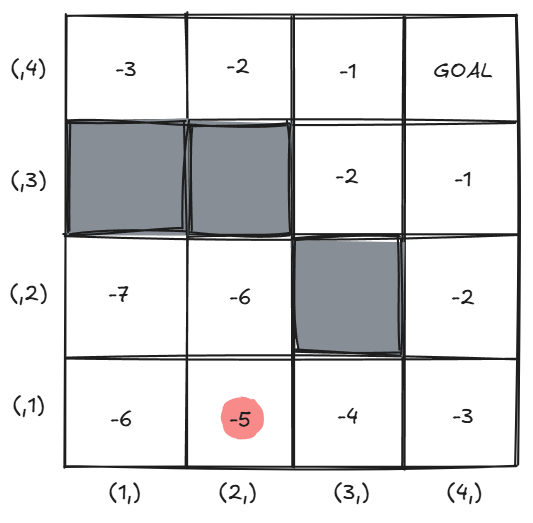
\includegraphics[width=0.5\textwidth]{./chapters/part-1/figures/emuexp.png}
	\caption{State utility map for in the MEU example.}
	\label{fig:emuexp}
\end{figure}

Let evidence $e$ be the current location of the AI agent. In this example, assume that the agent is at the red dot $(2,1)$. There are $4$ actions that the agent can take. They are listed below, together with the landing state and their associated probability.
\begin{eqnarray}
	a_1 &=& \mathrm{UP} \nonumber \\
	P\left((2,1)|a_1, e\right) &=& 0.2 \nonumber \\
	P\left((2,2)|a_1, e\right) &=& 0.6 \nonumber \\
	P\left((1,1)|a_1, e\right) &=& 0.1 \nonumber \\
	P\left((3,1)|a_1, e\right) &=& 0.1 \nonumber \\
	a_2 &=& \mathrm{LEFT} \nonumber \\
	P\left((2,1)|a_2, e\right) &=& 0.2 \nonumber \\
	P\left((2,2)|a_2, e\right) &=& 0.1 \nonumber \\
	P\left((1,1)|a_2, e\right) &=& 0.6 \nonumber \\
	P\left((3,1)|a_2, e\right) &=& 0.1 \nonumber \\
	a_3 &=& \mathrm{DOWN} \nonumber \\
	P\left((2,1)|a_3, e\right) &=& 0.7 \nonumber \\
	P\left((2,2)|a_3, e\right) &=& 0.1 \nonumber \\
	P\left((1,1)|a_3, e\right) &=& 0.1 \nonumber \\
	P\left((3,1)|a_3, e\right) &=& 0.1 \nonumber \\
	a_4 &=& \mathrm{RIGHT} \nonumber \\
	P\left((2,1)|a_4, e\right) &=& 0.2 \nonumber \\
	P\left((2,2)|a_4, e\right) &=& 0.1 \nonumber \\
	P\left((1,1)|a_4, e\right) &=& 0.1 \nonumber \\
	P\left((3,1)|a_4, e\right) &=& 0.6 \nonumber 
\end{eqnarray}
Notice that the output of an action is not deterministic. In practice, this can happen due to signal transmitting error, etc. Notice that the AI agent cannot move down at its current location. When ``DOWN'' action $a_3$ is taken, it will most likely run into the wall and stay where it is currently.

Using \eqref{eq:expected_utility}, the expected utility of $a_1$ can be calculated as follows.
\begin{eqnarray}
	EU(a_1|e) &=& 0.2\times(-5) + 0.6\times(-6) + 0.1\times(-6) + 0.1\times(-4) \nonumber \\
	&=& -5.6 \nonumber
\end{eqnarray}
and similarly, $EU(a_2|e) = -5.6$, $EU(a_3|e) = -5.1$ and $EU(a_4|e) = -4.6$. Using \eqref{eq:emu}, action $a_4$, i.e, move ``RIGHT'', is the rational decision.

The main challenges of the MEU include at least the following.
\begin{itemize}
	\item The utility of each state, $U(s_i)$, is often not obvious, and needs to be calculated by searching or learning.
	\item The probabilities $P(s|a_i,e)$ needs to be calibrated.
\end{itemize}
In the remaining of this chapter, the above two challenges will be addressed with different approaches.

\begin{mdframed}
\noindent \textbf{Are there alternative ways to calculate the utility of an action?}

The utility of an action is calculated by \eqref{eq:expected_utility} which intuitively makes sense. An AI agent who uses \eqref{eq:expected_utility} and \eqref{eq:emu} to make decisions seems rational. 

The question is, are there additional ways to calculate the utility of an action? For example, consider
\begin{eqnarray}
	U(a|e) &=& \mathrm{min}\left(\left\{U(s_i)|P(s_i|a,e) > 0\right\}\right) \nonumber
\end{eqnarray}
which counts for the ``worst utility'' an action may lead to. Can we use this utility instead of \eqref{eq:expected_utility} when evaluating an action?

This essentially addresses what an rational agent is. For that, the following \mync{axioms of utility theory} is defined.  
\begin{itemize}
	\item Orderability. Let there be two actions $a_1$ and $a_2$. Exactly on of the statements ``$a_1$ is preferred over $a_2$'', ``$a_1$ and $a_2$ are indifferent'', ``$a_2$ is preferred over $a_1$'' must be true. In other words, any action can be ranked.
	
	\item Transitivity. Let there be three actions $a_1$, $a_2$ and $a_3$, if $a_1$ is preferred over $a_2$, and $a_2$ over $a_3$, then $a_1$ must be preferred over $a_3$.
	
	\item Continuity. Let there be three actions $a_1$, $a_2$ and $a_3$, where $a_1$ is preferred over $a_2$, and $a_2$ over $a_3$. Define a new compound action $a_{1,3, p, 1-p}$, which randomly select $a_1$ with probability $p$ and $a_3$ with probability $1-p$. There must be such probability $p$ so that $a_2$ and $a_{1,3,p,1-p}$ are indifferent.
	
	\item Substituability. Let $a_1$ and $a_2$ be indifferent actions. Let $a_3$ be any action. Let $a_{1,3,p,1-p}$, $a_{2,3,p,1-p}$ be two compound actions with $p$ be any probability. Actions $a_{1,3,p,1-p}$ and $a_{2,3,p,1-p}$ must be indifferent.
	
	\item Monotonicity. Let $a_1$, $a_2$ be two actions and $a_1$ be preferred over $a_2$. Define two compound actions $a_{1,2,p_1,1-p_1}$, $a_{1,2,p_2,1-p_2}$. If $p_1 > p_2$ then $a_{1,2,p_1,1-p_1}$ is preferred over $a_{1,2,p_2,1-p_2}$.
	
	\item Decomposability. Compound actions can be nested or decomposed. For example, consider compound action $a_{1,2,p,1-p}$, where $a_2$ itself can be a compound action $a_2 = a_{21, 22, q,1-q}$. The compound action can be decomposed as follows $a_{1, 21, 22,p,(1-p)q,(1-p)(1-q)}$ which is indifferent with $a_{1,2,p,1-p}$.
\end{itemize}

Let $U(a)$ be the utility of an action $a$ which can be any action mentioned in the axioms of utility theory. The utility $U(a)$ must exist for every action, and its value must be able to reflect the preference, i.e., if $U(a_1) > U(a_2)$, it will prefer $a_1$ over $a_2$, and if $U(a_1) = U(a_2)$, it is indifferent between $a_1$ and $a_2$.

It can be proved that for an compound action, its utility is 
\begin{eqnarray}
	U\left(a_{1,2,..., n,p_1,p_2,..., p_n}\right) &=& \sum_n p_i U(a_i) \nonumber
\end{eqnarray}

It is obvious that utility function is not unique. For example, given utility function $U(a)$,
\begin{eqnarray}
U\textprime (a) &=& \alpha U(a) + \beta, \alpha > 0 \nonumber
\end{eqnarray}
is also a valid utility calculation.

\end{mdframed}

\subsection{Utility Function}

The utility of an action $U(a|e)$, for example \eqref{eq:expected_utility}, is an example of a \mync{utility function} which maps an action to a real number. Notice that as mentioned earlier, \eqref{eq:expected_utility} is not the unique way of calculating the utility of an action that fulfills the axioms of utility theory. Different utility functions are briefly discussed in this section. The calculation of utility functions for each action at each state is often known as \mync{preference elicitation}.

The utility of a state can be taken as an extension to the utility of an action. For example, in \eqref{eq:expected_utility} the utility of a state $U(s)$ is often calculated as the maximum value of utility functions among all probable actions on that state, i.e.,
\begin{eqnarray}
	U(s) &=& \max_i \left(EU(a_i|e)\right) \label{eq:stateutility}
\end{eqnarray}
where $a_i$ is any probable action that can be taken at state $s$. Using \eqref{eq:stateutility}, the utility of states can be calculated from the utility of actions.


The calculation of utility functions can be challenging. For example, consider $U(a|e)$ given by \eqref{eq:expected_utility}. The transaction probability $P(s|a,e)$ and the state utility $U(s)$ are usually unknown in the beginning and need to be calibrated. There are different ways to calibrate their values. In the later Sections \ref{sec:mdp} and \ref{sec:pomdp}, the calculation of utility functions in Markov decision process, one of the most widely used decision making model, will be introduced in more details.

\section{Decision Network}

\section{Markov Decision Process} \label{sec:mdp}

\subsection{State and Policy}

State.

Policies.

Optimal policy.

Utility of a state.

\subsection{Value Iteration}

Bellman equation and convergence.

\subsection{Policy Iteration}

\section{Partially Observable MDP} \label{sec:pomdp}

\section{Game Theory}

Multi-agent control system.